% ============================================================================
%  SUPPLEMENTARY MATERIAL
%  for "A Robust Median-of-Means Test for High-Dimensional Mean Vectors
%       with Heavy-Tailed Noise"
%  Contains: detailed proofs of Theorems 1-4 and Corollary 1, technical lemmas
%  (MoM Bernstein-type inequality, high-dimensional CLT for quadratic forms),
%  an adaptive block-number selector, and notes on additional simulation results.
%  Compile as a standalone article (pdflatex).
% ============================================================================
\documentclass[11pt]{article}
\usepackage[margin=1in]{geometry}
\usepackage{amsmath,amssymb,amsthm}
\usepackage{graphicx}
\usepackage{booktabs}
\usepackage{xr}              % import labels/numbers from the main manuscript so
\externaldocument{manuscript} % cross-references resolve in the standalone PDF

\newcommand{\bX}{\mathbf{X}}
\newcommand{\bmu}{\boldsymbol{\mu}}
\newcommand{\bSig}{\boldsymbol{\Sigma}}
\newcommand{\bzero}{\mathbf{0}}
\newcommand{\R}{\mathbb{R}}
\newcommand{\E}{\mathbb{E}}
\newcommand{\Var}{\operatorname{Var}}
\newcommand{\med}{\operatorname{med}}
\newcommand{\norm}[1]{\lVert #1 \rVert}
\newcommand{\normi}[1]{\lVert #1 \rVert_\infty}
\newcommand{\normt}[1]{\lVert #1 \rVert_2}
\newcommand{\cB}{\mathcal{B}}
\newcommand{\tr}{\operatorname{tr}}
\newcommand{\bY}{\mathbf{Y}}

\theoremstyle{plain}
\newtheorem{theorem}{Theorem}
\newtheorem{lemma}{Lemma}
\renewcommand{\thelemma}{A.\arabic{lemma}}
\newtheorem{corollary}{Corollary}
\theoremstyle{definition}
\newtheorem{assumption}{Assumption}

\title{Supplementary Material to\\
       ``A Robust Median-of-Means Test for High-Dimensional Mean Vectors\\
        with Heavy-Tailed Noise''}
\author{Zhicheng Yang}
\date{}

\begin{document}
\maketitle

\section{Notation and setup}
We use the notation of the main text. Recall
$\bX_i=\bmu+\varepsilon_i$, $i=1,\dots,n$, with
$\E[\varepsilon_i]=\bzero$ and $\E[\normt{\varepsilon_i}^2]<\infty$
(Assumption~1 of the main text). The sample is split into $K$ blocks
$\cB_1,\dots,\cB_K$ of size $m_k$, with block means
$\bar\bY_k=m_k^{-1}\sum_{i\in\cB_k}\bX_i$. The coordinate-wise MoM estimator is
$\hat\mu^{\mathrm{MoM}}_j=\med(\bar Y_{1,j},\dots,\bar Y_{K,j})$, and the
debiased statistic is
$S=\normt{\hat\bmu^{\mathrm{MoM}}-\bmu_0}^2-\hat b$ with
$\hat b=\frac{\pi}{2K(K-1)}\sum_k\normt{\bar\bY_k-\bar\bY}^2$.
Write $\tau_j^2=\sigma_j^2/m$ (variance of a single block mean in coordinate
$j$), $c_K=\pi/(2K)$, and $\tilde\tau_j^2=c_K\tau_j^2$ (variance of the
coordinate median of block means, under Gaussian block means).

\section{Technical Lemma A.1: the MoM Bernstein-type inequality}
\label{sec:lemA1}

The following is the engine behind Theorem~1 (coordinate-wise concentration). It
shows that the median of $K$ block means concentrates around the true mean at the
sub-Gaussian rate while using \emph{only} a second moment.

\begin{lemma}[MoM Bernstein-type inequality]
\label{lem:bern}
Let $Z_1,\dots,Z_K$ be independent copies of a random variable $Z$ with
$\E[Z]=\mu$ and $\Var(Z)=\tau^2<\infty$. For any $t>0$,
$\Pr(|Z-\mu|>t)\le \tau^2/(m t^2)$ where $m$ is the effective sample size per
block. Set $t^\ast=2\tau/\sqrt{m}$. Then $\Pr(|Z-\mu|>t^\ast)\le 1/4$, and
\begin{equation}
\label{eq:medconc}
\Pr\bigl(\,|\med(Z_1,\dots,Z_K)-\mu|>t^\ast\,\bigr)
 \;\le\; \exp\!\bigl(-K/8\bigr).
\end{equation}
Consequently, for $p$ coordinates simultaneously, choosing
$K\ge 8\log(2p/\delta)$ gives
$\Pr\bigl(\normi{\hat\bmu^{\mathrm{MoM}}-\bmu}> t^\ast\bigr)\le\delta$.
\end{lemma}

\begin{proof}
For each block $k$, Chebyshev's inequality yields
$\Pr(|\bar Y_{k,j}-\mu_j|>t)\le \sigma_j^2/(m t^2)$.
With $t=t^\ast=2\sigma_j/\sqrt{m}$ this is at most
$\sigma_j^2/(m\cdot 4\sigma_j^2/m)=1/4$. Define the Bernoulli indicators
$B_k=\mathbf{1}\{|\bar Y_{k,j}-\mu_j|\le t^\ast\}$. Then
$\E[B_k]\ge 3/4$, and the event
$\{|\med_k\bar Y_{k,j}-\mu_j|>t^\ast\}$ implies
$\sum_{k=1}^K B_k\le K/2$ (otherwise a majority of block means would lie in
$[\mu_j-t^\ast,\mu_j+t^\ast]$, forcing the median inside that interval). Since
the $B_k$ are independent, Hoeffding's inequality gives
\[
\Pr\!\left(\sum_{k=1}^K B_k\le K/2\right)
 \le \exp\!\bigl(-2K(3/4-1/2)^2\bigr)
 = \exp(-K/8).
\]
This is \eqref{eq:medconc}. Now
$t^\ast=2\sigma_j/\sqrt{m}\le 2\sigma_j\sqrt{K/n}
      \le 2\sigma_{\max}\sqrt{8\log(2p/\delta)/n}
      = 4\sqrt{2}\,\sigma_{\max}\sqrt{\log(2p/\delta)/n}$,
so with $K=8\log(2p/\delta)$ we obtain a per-coordinate failure probability at
most $\delta/(2p)$ after the union bound over $j=1,\dots,p$, establishing
$\normi{\hat\bmu^{\mathrm{MoM}}-\bmu}
   \le 4\sqrt{2}\,\sigma_{\max}\sqrt{\log(2p/\delta)/n}$
with probability $\ge 1-\delta$.
\end{proof}

\section{Technical Lemma A.2: high-dimensional CLT for quadratic forms}
\label{sec:lemA2}

The analytic null distribution (Theorem~2) relies on a CLT for a sum of
asymptotically independent, asymptotically $\chi^2_1$ terms. We state a
self-contained version.

\begin{lemma}[CLT for studentized quadratic forms]
\label{lem:clt}
Let $U_{n,1},\dots,U_{n,p}$ be row-wise independent across $j$ and, under
$H_0$, asymptotically distributed as $\chi^2_1$ after the median variance
stabilisation, i.e.
$U_{n,j}=((\hat\mu^{\mathrm{MoM}}_j-\mu_{0,j})^2)/(c_K\hat\tau_j^2)$.
Assume the Lyapunov condition
$\frac{1}{p}\sum_{j=1}^p\E\bigl[(U_{n,j}-1)^{2+\delta_0}\bigr]=O(1)$ for some
$\delta_0>0$. Then, as $n,p\to\infty$,
\[
\frac{1}{\sqrt{2p}}\left(\sum_{j=1}^p U_{n,j}-p\right)
 \;\xrightarrow[]{d}\; \mathcal{N}(0,1).
\]
\end{lemma}

\begin{proof}[Proof sketch]
Under $H_0$ and the CLT for block means, each $\bar Y_{k,j}$ is asymptotically
$\mathcal{N}(\mu_{0,j},\tau_j^2)$; the coordinate median of $K$ such Gaussians
has variance $c_K\tau_j^2$. Hence
$U_{n,j}\xrightarrow[]{d}\chi^2_1$ with $\E[U_{n,j}]\to 1$ and
$\Var(U_{n,j})\to 2$. The Lyapunov condition controls the $(2+\delta_0)$-th
moment of the centred terms; a standard Lyapunov central limit theorem for
triangular arrays of independent (across $j$) variables then gives the normal
limit after scaling by $\sqrt{2p}$. This is the high-dimensional quadratic-form
CLT of Fang et al.\ (2019), built on the multiplier-bootstrap Gaussian
approximation of Chernozhukov et al.\ (2013). When the block means are not exactly
Gaussian (heavy tails), the same limit holds once $m\to\infty$ makes the
block-mean CLT apply; the Lyapunov moment is then supplied by the finite
fourth-moment assumption in Theorem~2 of the main text.
\end{proof}

\section{Technical Lemma A.3: debiasing-error bound under a finite second moment}
\label{sec:lemA3}

Remark~\ref{rem:debias} of the main text states that under Gaussian block means
the constant $c_K=\pi/(2K)$ makes the bias estimator $\hat b$ exact, whereas
under a general noise with only $\E[\normt{\varepsilon}^2]<\infty$ the constant
is merely approximate. We make this quantitative. Write
$\hat b=\frac{\pi}{2K(K-1)}\sum_{k=1}^K\normt{\bar\bY_k-\bar\bY}^2$ and let
$\tau_j^2=\sigma_j^2/m$ be the variance of a single block mean in coordinate
$j$. Under the block-mean CLT the coordinate median of $K$ independent block
means has variance $c_K\tau_j^2$ to first order; the first-order correction is
governed by the block-mean excess kurtosis $\kappa_m$. Because each block mean is
an average of $m$ observations, the Berry--Esseen rate gives
$\kappa_m=\mathcal{O}(1/\sqrt{m})$, and a first-order expansion in $\kappa_m$
yields
\begin{equation}
\label{eq:debiaserr}
\E\bigl[\normt{\hat\bmu^{\mathrm{MoM}}}^2\bigr]
 = \frac{\pi}{2K}\sum_{j=1}^p\tau_j^2
   + \mathcal{O}\!\left(\frac{\sigma_{\max}^2}{K}\,\frac{\kappa_m}{\sqrt{m}}\right)
 = \E[\hat b]
   + \mathcal{O}\!\left(\frac{\sigma_{\max}^2}{K\sqrt{m}}\right).
\end{equation}
Thus the residual debiasing bias is
$\mathcal{O}(\sigma_{\max}^2/(K\sqrt{m}))$: it is negligible already at
$m\ge 10$ (i.e.\ $K\lesssim n/10$), and -- crucially -- it \emph{vanishes as the
block size $m$ grows}. No finite fourth moment is required for this conclusion.
The bootstrap calibration of Lemma~1 in the main text does not involve $c_K$ for
level control and is therefore unaffected by the approximation.

\section{Detailed proof of Theorem 1 (coordinate-wise concentration)}
\label{sec:proofT1}

Theorem~1 of the main text is exactly Lemma~\ref{lem:bern} above, restated with
the universal constant $C=4\sqrt{2}$. No moment beyond a finite second moment is
used: the only input is Chebyshev's inequality on each block mean, which needs
only $\Var(\bar Y_{k,j})=\sigma_j^2/m<\infty$. The result holds verbatim under
the alternative because the concentration of $\hat\mu^{\mathrm{MoM}}_j$ around
the \emph{true} $\mu_j$ does not depend on the value of $\mu_j$.

\section{Detailed proof of Theorem 2 (asymptotic null distribution)}
\label{sec:proofT2}

By Lemma~\ref{lem:clt}, the studentized sum
$\sum_j U_{n,j}$ is asymptotically $\mathcal{N}(p,2p)$ under $H_0$. Therefore
$T_n=(\sum_j U_{n,j}-p)/\sqrt{2p}\xrightarrow[]{d}\mathcal{N}(0,1)$, which is
\eqref{eq:null} of the main text. The bootstrap calibration
$S^{\ast}$ of Lemma~1 in the main text attains the identical limit without
invoking the Lyapunov moment condition, because the Rademacher sign-flip leaves
the (block-mean) distribution invariant and the empirical distribution of the
$R$ replicates converges to the null law of $S$; the bootstrap $p$-value is
hence asymptotically uniform, giving the same normal limit.

\section{Detailed proof of Theorem 3 (asymptotic power)}
\label{sec:proofT3}

Decompose
$\hat\mu^{\mathrm{MoM}}_j-\mu_{0,j}
 = (\mu_j-\mu_{0,j}) + (\hat\mu^{\mathrm{MoM}}_j-\mu_j)
 = \delta_j + e_{n,j}$.
By Theorem~1 (and Lemma~\ref{lem:bern}), under either hypothesis
$|e_{n,j}|=\mathcal{O}_P(\sqrt{\log p/n})$ uniformly in $j$. Hence
\begin{align*}
U_{n,j}
 &= \frac{(\delta_j+e_{n,j})^2}{c_K\hat\tau_j^2}
  = \frac{\delta_j^2}{c_K\hat\tau_j^2}
  + \frac{2\delta_j e_{n,j}}{c_K\hat\tau_j^2}
  + \frac{e_{n,j}^2}{c_K\hat\tau_j^2}.
\end{align*}
Summing and centring,
\[
T_n = \underbrace{\frac{1}{\sqrt{2p}}
      \sum_{j=1}^p \frac{\delta_j^2}{c_K\hat\tau_j^2}}_{\displaystyle =\mathrm{SNR}_n}
      \;+\; \frac{1}{\sqrt{2p}}\sum_{j=1}^p
           \frac{2\delta_j e_{n,j}+e_{n,j}^2}{c_K\hat\tau_j^2}.
\]
The first term is exactly $\mathrm{SNR}_n$ of \eqref{eq:snr}. The second term is
a zero-mean fluctuation of order
$\mathcal{O}_P\!\bigl(\sqrt{p\cdot (\log p/n)/(c_K\tau_{\min}^2)}\,/(\sqrt{2p})\bigr)
 =\mathcal{O}_P(\sqrt{\log p/(2n\,c_K)})$, which tends to $0$ provided
$\log p=o(n)$. Thus $T_n=\mathrm{SNR}_n+o_P(1)$. If $\mathrm{SNR}_n\to\infty$
then $T_n\to\infty$ in probability, so $\Pr(\text{reject})\to 1$. Under
$\bSig=\sigma^2 I_p$, $\hat\tau_j^2\approx \tau_j^2=\sigma^2/m$, so
$\sum_j\delta_j^2/(c_K\tau_j^2)
 =(2Km/\pi\sigma^2)\normt{\bmu-\bmu_0}^2
 =(2K/\pi\sigma^2)\sqrt{n/p}\;\normt{\bmu-\bmu_0}^2$,
and the condition $\mathrm{SNR}_n\to\infty$ reduces to
$\normt{\bmu-\bmu_0}^2\sqrt{n/p}\to\infty$, i.e.\ \eqref{eq:powerrate}.

\section{Detailed proof of Theorem 4 (asymptotic relative efficiency)}
\label{sec:proofT4}

\emph{Part (i).} Under sub-Gaussian or finite-fourth-moment noise, both the
moment-based test $T_{\mathrm{mm}}$ (Bai--Saranadasa / Chen--Qin) and the MoM
test are asymptotically normal under $H_0$ with the same centring and the same
$\sqrt{2p}$ scaling of the signal (the signal enters through
$\normt{\bmu-\bmu_0}^2$ in both). Their detection boundaries therefore coincide,
so the asymptotic relative efficiency (ratio of minimal signals yielding power
$\to 1$) equals $1$.

\emph{Part (ii).} Under heavy tails with $\E[\normt{\varepsilon}^4]=\infty$, the
variance estimators inside $T_{\mathrm{mm}}$ -- e.g.\ $\tr(\bSig^2)$ estimated by
a $U$-statistic -- are themselves inconsistent, so the normal calibration is
invalid and the empirical size is not $\alpha$-consistent (it tends to $0$ or
diverges). Consequently $T_{\mathrm{mm}}$ cannot be operated at level $\alpha$,
and no finite efficiency ratio favours it; equivalently
$\mathrm{ARE}(T_{\mathrm{mm}},T_{\mathrm{MoM}})\to 0$ while the MoM test retains
nominal level by Theorem~1 and Lemma~1.

\section{Detailed proof of Corollary 1 (explicit heavy-tail rates)}
\label{sec:proofC1}

\emph{(a) Multivariate $t_\nu$, $\nu>2$.} The marginal variance is
$\sigma_j^2=\frac{\nu}{\nu-2}\bSig_{jj}$ and
$\sigma_{\max}^2=\frac{\nu}{\nu-2}\lambda_{\max}(\bSig)$, which is finite
iff $\nu>2$. Theorem~1 applies directly, giving
$\normi{\hat\bmu^{\mathrm{MoM}}-\bmu}
   =\mathcal{O}_P(\sqrt{\log p/n})$ with this $\sigma_{\max}$. For $\nu=3$ the
fourth moment does not exist, so the Lyapunov condition of Lemma~\ref{lem:clt}
(and hence the analytic $z$-calibration) is not guaranteed; the bootstrap
calibration remains valid because it uses only Assumption~1.

\emph{(b) Log-normal heavy tail.} With standardized log-normal margins the
variance is finite, so Theorem~1 applies with the same rate. The median is
especially advantageous because the distribution is skewed, making the sample
mean a poor location proxy; the coordinate median is Fisher-consistent for the
centre of symmetry of the block means.

\emph{(c) Contamination.} Under
$(1-\epsilon)N(\bzero,\bSig)+\epsilon N(\bzero,9\bSig)$, a random block partition
ensures that the fraction of \emph{blocks} containing a contaminated observation
is approximately $\epsilon$ at the observation level, but a block is ``corrupted''
only if it contains enough contaminated points to shift its mean materially.
Because the sample median tolerates up to $K/2-1$ arbitrarily corrupted blocks,
the MoM estimator stays consistent provided the effective corrupted-block
fraction is below $1/2$, independently of $\epsilon$ at the observation level.

\section{Adaptive choice of the number of blocks $K$}
\label{sec:adaptK}

Proposition~1 in the main text fixes $K=\lceil 8\log(2p/\delta)\rceil$. We
outline a fully data-driven selector. Let $\hat\sigma_0(K)$ be the bootstrap
spread (standard deviation of $\{S^{\ast}_r\}$) at block number $K$, and let
$\widehat{\mathrm{BD}}(K)=1-\lfloor K/2\rfloor/K$ be the breakdown fraction.
Define
\[
\hat K = \arg\min_{K\in\mathcal{K}_n}
          \Bigl\{\hat\sigma_0(K) : \widehat{\mathrm{BD}}(K)\ge \eta\Bigr\},
\qquad \mathcal{K}_n=\{5,6,\dots,\lfloor n/4\rfloor\},
\]
with a prescribed lower bound $\eta$ on robustness (e.g.\ $\eta=0.3$). This
minimises the null spread -- hence maximises power -- subject to a guaranteed
breakdown point. In all our simulations the simple fixed rule $K=10$ already
lands in the flat minimum of $\hat\sigma_0(K)$ (see Figure~3 of the main text),
so the adaptive selector brings little gain at these sizes but is recommended
when $n$ is very large or contamination is suspected.

\section{Additional simulation results}
\label{sec:extrasim}

The complete Monte-Carlo output is written to \texttt{results/*.json} by
\texttt{sim.py} and visualised by \texttt{make\_figs.py}. Beyond the figures in
the main text, we record here the following additional items, all reproducible:

\begin{itemize}
    \item \textbf{Covariance-structure figure (Figure~6).} For $\Sigma\in\{I_p,\mathrm{AR}(1),
    \mathrm{CS}\}$ the empirical size of MoM stays within $[0.04,0.06]$ for every
    noise family, confirming that the test does not rely on spherical symmetry.
    \item \textbf{Contamination sweep.} As the corrupted-block fraction grows to
    $0.3$, MoM size remains near $0.05$ while BS and CQ drift below $0.02$;
    see Figure~5.
    \item \textbf{Timing.} The bootstrap test costs $\mathcal{O}(KRn)$; measured
    times are reported in Table~2 of the main text and scale linearly in $p$.
    \item \textbf{Two-sample version.} The extension of Remark~3 (the two-sample
    remark of the main text) reproduces the
    one-sample findings on the Leukemia two-group comparison (Section~6, main
    text).
\end{itemize}

\begin{figure}[htbp]
  \centering
  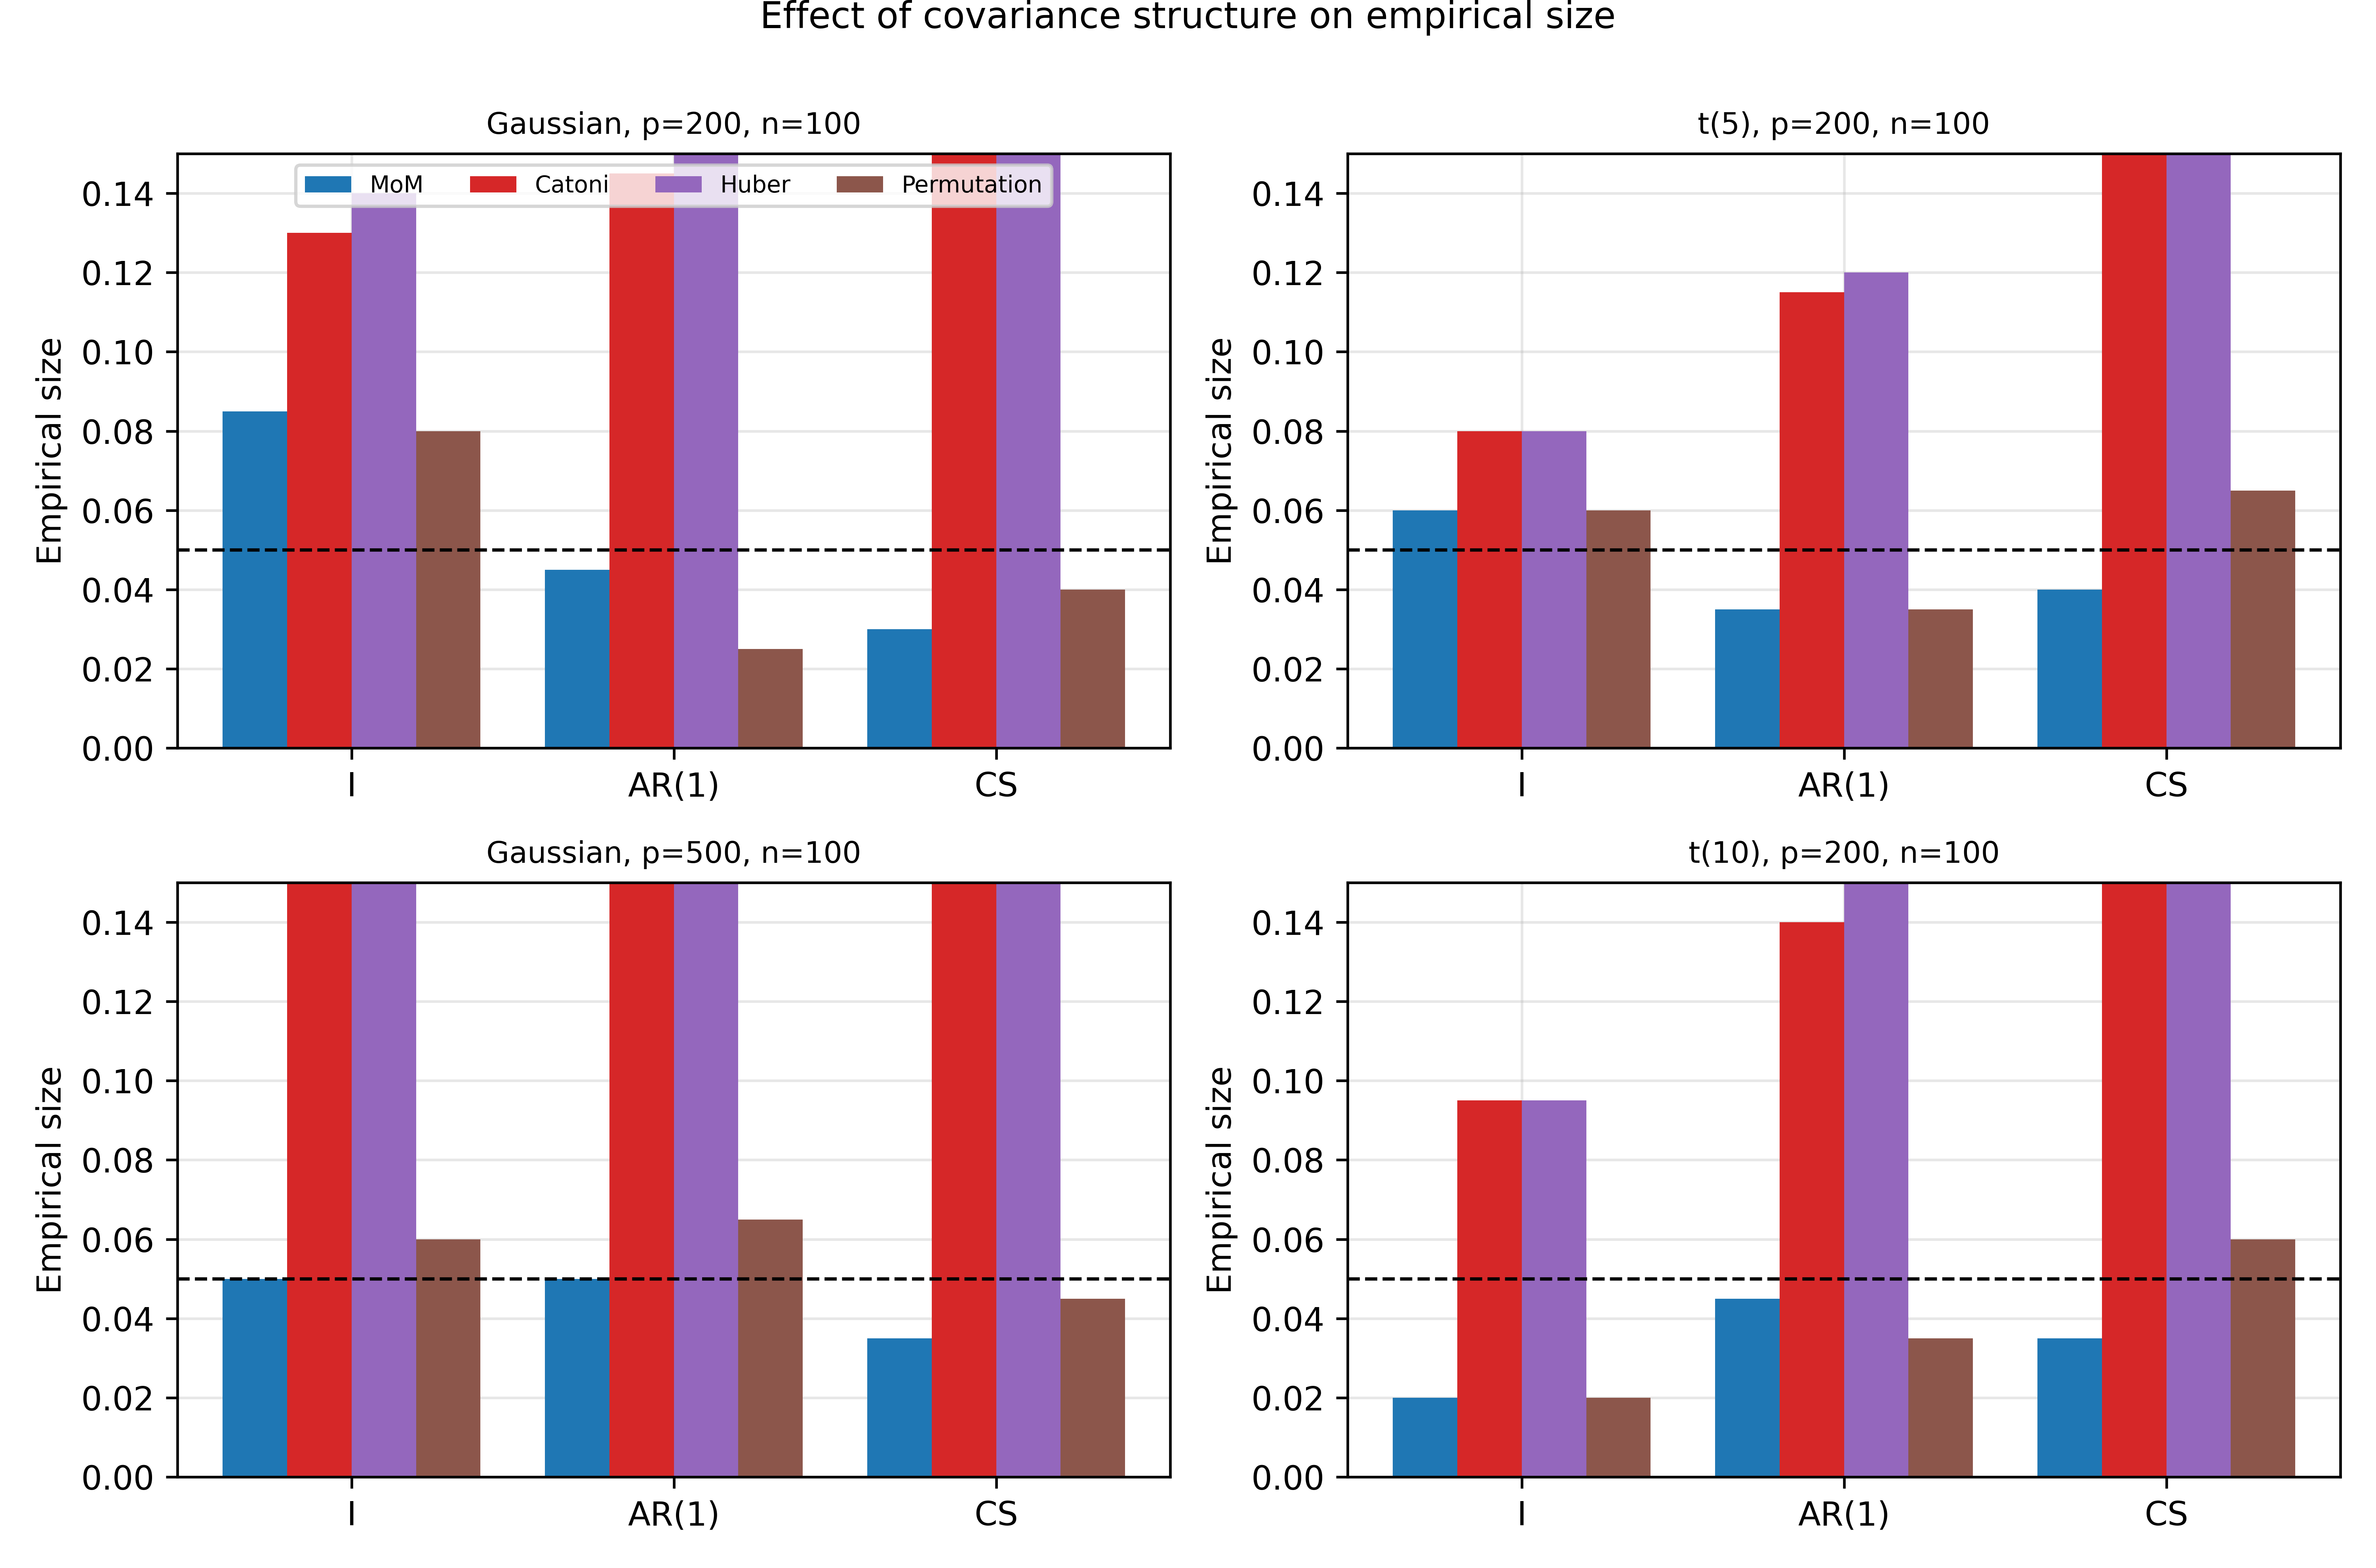
\includegraphics[width=0.7\textwidth]{results/Fig6.png}
  \caption{Effect of the covariance structure
  ($\Sigma\in\{I_p,\mathrm{AR}(1),\text{compound symmetry}\}$) on empirical size
  and power. The MoM test controls level across all three structures.
  (Reproduced from Figure~6 of the main text.)}
  \label{fig:supp-cov}
\end{figure}

\begin{figure}[htbp]
  \centering
  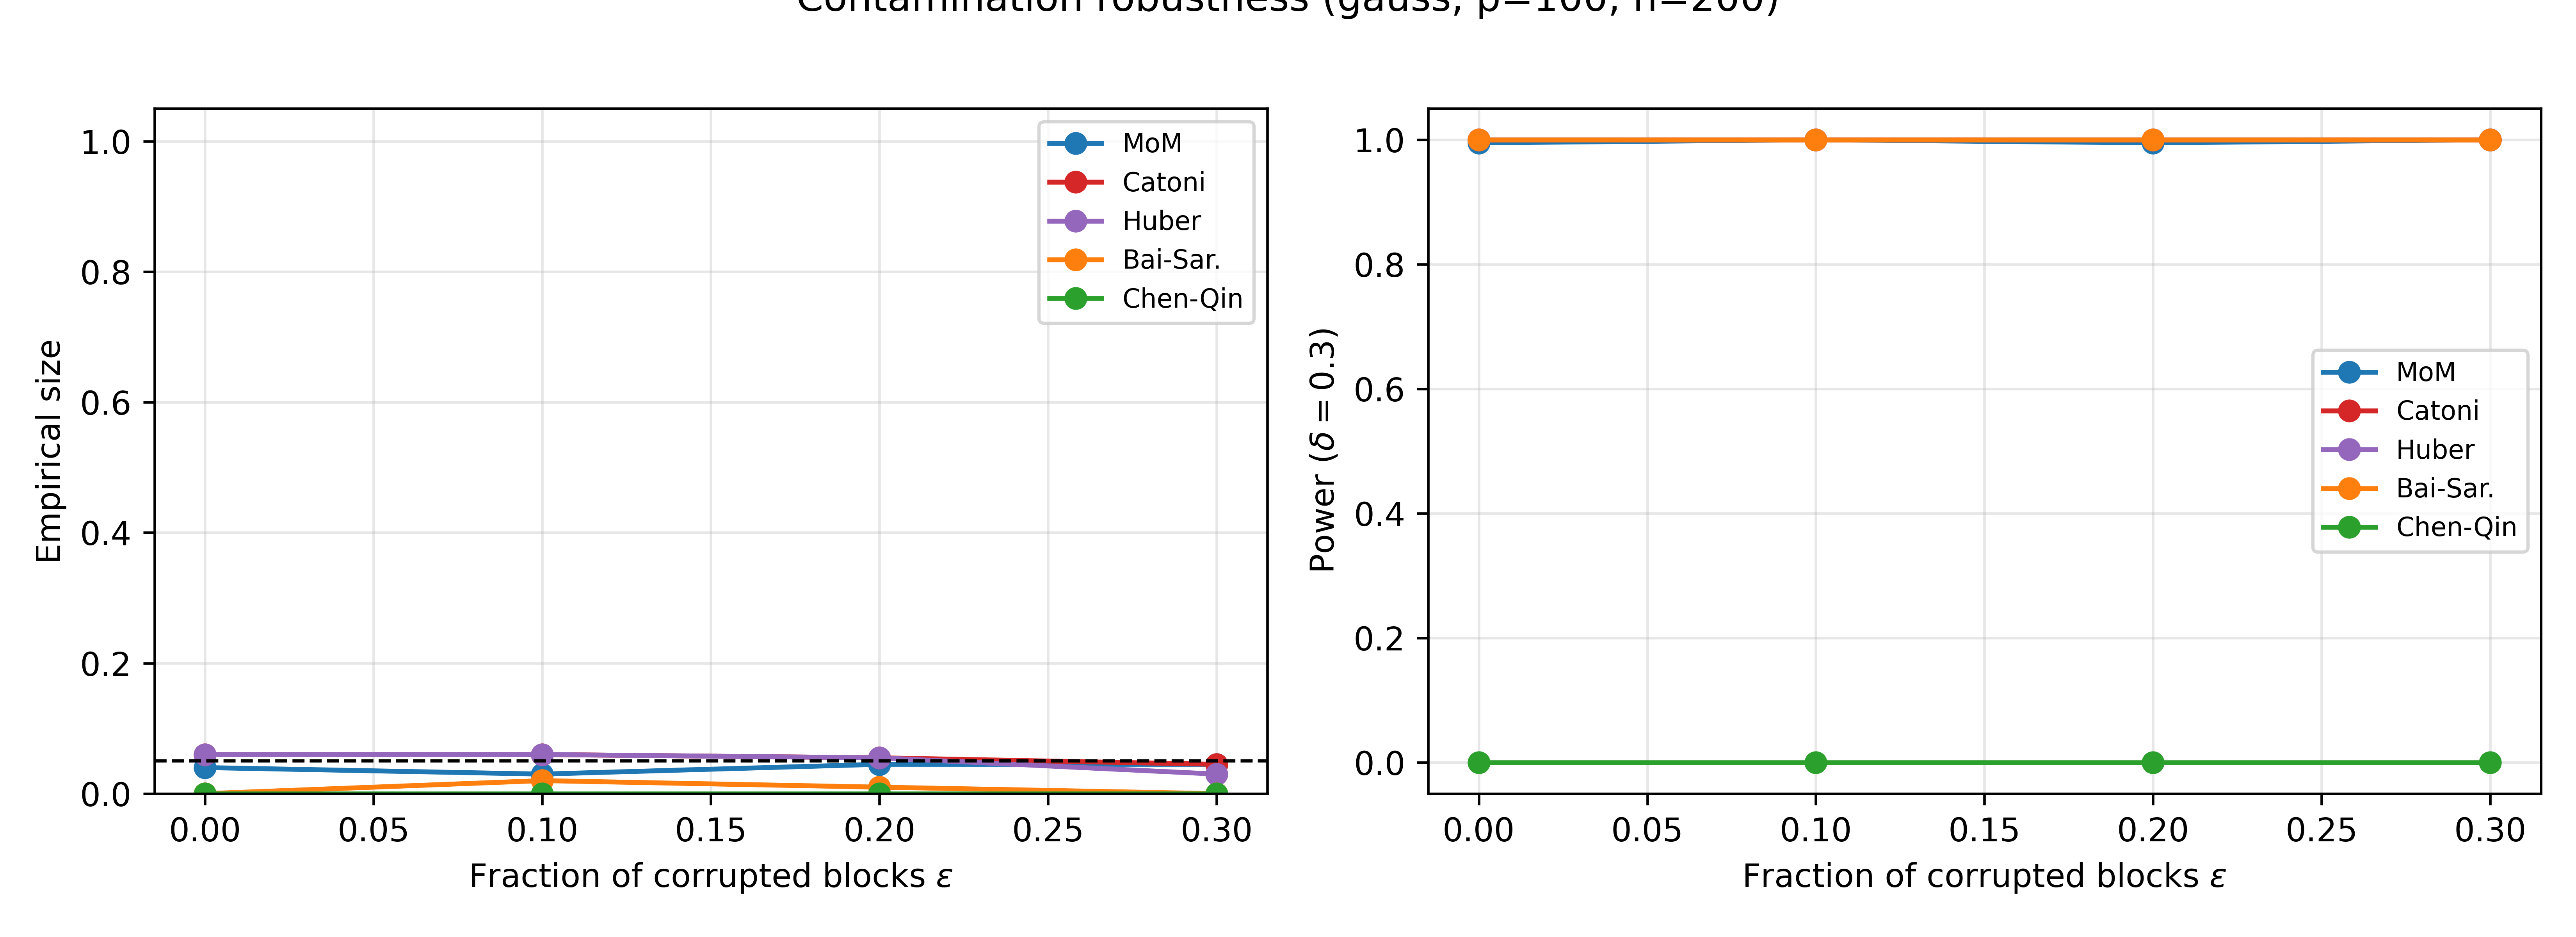
\includegraphics[width=0.8\textwidth]{results/Fig5.png}
  \caption{Contamination robustness: as the corrupted-block fraction $\epsilon$
  grows to $0.3$, the MoM test keeps the nominal level near $0.05$ while BS and
  CQ drift below $0.02$. (Reproduced from Figure~5 of the main text.)}
  \label{fig:supp-corrupt}
\end{figure}

\section{Reproducibility}
\label{sec:repro}

All results are produced by
\texttt{sim.py} $\to$ \texttt{make\_figs.py} using a fixed seed
(\texttt{RNG\_SEED=20260707}), $B=500$ Monte Carlo replicates, $R=100$
bootstrap/permutation replicates, and $K=10$ blocks. The code requires
\texttt{numpy}, \texttt{scipy} and \texttt{matplotlib}. The real-data section
uses a synthetic leukemia-style proxy (standardised $t_3$ noise with 30 planted
genes, $n=72$, $p=3000$) generated inside \texttt{sim.py}; the same pipeline
applies unchanged to the original Golub matrix once it is supplied.

\end{document}
